We have thus far described the likelihood,
$\Prob(X | N, \ell, f)$, and specified the prior, $\Prob(N, \ell, f)$. 
For simplicity, latent variables $\ell$, $f$ without subscripts  
denote the entire triangular array. We seek the posterior distribution 
$\Prob(N, \ell, f | X)$. In most nontrivial probabilistic models, including ours, the exact posterior distribution is intractable.

Markov chain Monte Carlo (MCMC) is a common approach for approximating
posterior distributions by constructing a stochastic process on the parameter space whose stationary distribution is the true posterior. 
However, its computational cost is prohibitively large for
large scale astronomical surveys. Instead, we propose to construct an approximate posterior using variational inference, resulting in a procedure that is several orders of magnitude faster than MCMC.

Variational inference\cite{Blei_2017_vi_review, Jordan_intro_vi, Wainwrite_graph_models_vi}
posits a family of distributions $\mathcal{Q}$ and seeks
the distribution $q^*\in \mathcal{Q}$ that is closest to the true posterior
in $\KL$ divergence. Suppose the family of distributions $\mathcal{Q}$ is parameterized by a real-valued vector $\eta$. The objective is 
\begin{align}
   \eta^* &= \arg \min_{\eta} \Big\{ \mathrm{KL}\Big[\,q_\eta(N, \ell, f | X)\, \| \,\Prob(N, \ell, f | X )\,\Big]\Big\} 
   \label{eq:kl_objective}
\end{align}

We note that minimizing the $\KL$ divergence is equivalent to maximizing the ELBO (evidence lower bound), defined as 
\begin{align}
    \mathcal{L}(\eta) = \Expect\Big[\log\Prob(X, N, \ell, f) - \log q_\eta(N, \ell, f | X)\Big]
    \label{eq:elbo}
\end{align}

\subsection{The variational distribution}
We now describe our family of distributions $\mathcal{Q}$. 
In the classical variational inference setup, 
$q_\eta$ depends on data $X$ only through the optimization objective 
(so $q_\eta(N, \ell, f | X)$,
becomes $q_\eta(N, \ell, f)$ with no dependence on $X$). 
Here, we take an amortized approach, where 
$q_\eta$ takes input data $X$ and returns a distribution on the 
latent variables $(N, \ell, f)$. This mapping is encoded by  
neural network, so the variational parameter $\eta$ in equation~\ref{eq:kl_objective} are the neural network weights. 
In the ensuing subsections, we detail the construction of our variational 
distribution. 

\subsubsection{The factorization}
To make the objective in equation~\ref{eq:kl_objective} tractable in most 
applications, the family $\mathcal{Q}$ is restricted to probability distributions 
such that the latent variables have limited conditional dependencies. In the most extreme case, mean-field variational inference, the latent variables are assumed to fully factorize in the approximate posterior. 

Our factorization takes a spatial structure: we first decompose the full 
$H \times W$ image into disjoint $s \times s$ tiles. 
Independently for each tile,
we infer the number, locations, and fluxes of all stars falling in that tile.
Let $k = 1, ..., K$ index the tile. Then we
denote the number of stars on tile $k$ by $N^k$;
the locations by $\ell^k = (\ell_{N, i}^k)_{i \leq N}$; 
the fluxes $f^k = (f_{N, i}^k)_{i \leq N}$. While locations on the 
full image $\ell_{N, i}$ are in $[0, H] \times [0, W]$, 
locations on the tiles are parameterized such that 
$\ell^k_{N, i}\in[0, s] \times [0, s]$. A schematic 
of our tiling is shown in figure~\ref{fig:ex_tiles}. 

\begin{figure}
    \centering
    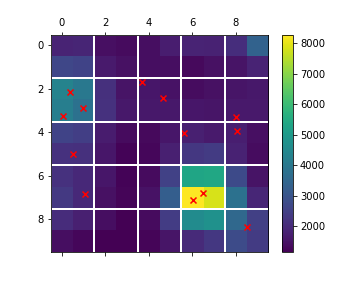
\includegraphics[width = 0.5\textwidth]{figures/example_tiled.png}
    \caption{Tiling a 10 x 10 image into 2 x 2 patches. }
    \label{fig:ex_tiles}
\end{figure}

Note that there is a bijection between latent variables on each tile and latent variables on the full image (locations on the full image map to locations on image tiles and vice-versa). Thus, a variational distribution for the latent variables on tiles induces a variational distribution for latent variables on the full image. 

In summary, we construct a distribution for latent variables on each tile that factorize over tiles: 
\begin{align}
    q((N^k, \ell^k, f^k)_{k = 1}^K|X) = \prod_{k = 1}^K q_\eta(N^k, \ell^k, f^k | X). 
\end{align}
If $f$ is the mapping from tile latent variables to full image latent variables, 
then the variational distribution on the full image latent variables 
$(N, \ell, f)$ is given by 
\begin{align}
    (N, \ell, f) &\stackrel{d}{=} f((N^k, \ell^k, f^k)_{k = 1}^K), \notag \\  
        &\text{where } (N^k, \ell^k, f^k)_{k = 1}^K \sim \prod_{k = 1}^K q_\eta(N^k, \ell^k, f^k | X). 
\end{align}

\subsubsection{Distributions on image tiles}
We describe the distribution on each tile, $q_\eta(N^k, \ell^k, f^k | X)$. 
Dropping the tile index $k$ in this subsection,
\begin{align}
    N &\sim \text{Categorical}(\omega; 0, ..., N_{max}) \label{eq:var_distr_n}\\
	\ell_{N, i} &\sim \text{LogitNormal}(\mu_{\ell_{N, i}}, \text{diag}(\nu_{\ell_{N, i}}) )\label{eq:var_distr_loc}\\
	f^b_{N, i} &\sim \text{LogNormal}(\mu_{f^b_{N, i}}, \sigma^2_{f^b_{N, i}}) \label{eq:var_distr_f}
\end{align}
for $i = 1, ..., N$; $N = 1, ..., N_{max}$, and the latent variables also fully factorize within each tile. Note that in the true posterior, $N$ has support on the nonnegative integers; in practice, we truncate at an $N_{max}$ large. 

\subsubsection{Neural network architecture}
The parameters of the variational distribution (equations~\ref{eq:var_distr_n}-\ref{eq:var_distr_f}) are given by the output of a neural network. The neural network takes as input the $s \times s$ tile, plus some surrounding pixels. 
For the problem of cataloging crowded starfields, we take $s = 2$ and pad the tile with three pixels. The architecture is shown schematically in figure~\ref{fig:starnet_arch}. 

\begin{figure}[h]
    \centering
    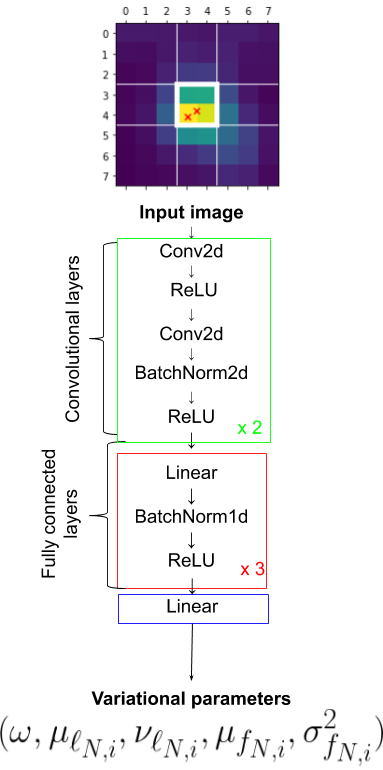
\includegraphics[width=0.4\textwidth]{figures/starnet_archetecture2.png}
    \vspace{-0.5cm}
    \caption{The neural network returning parameters for the variational distribution on each 2 x 2 image tile.}
    \label{fig:starnet_arch}
\end{figure}

Consider the output dimension of the neural network. The categorical parameter $\omega$ lies on the 
simplex and has dimension $N_{max} + 1$; for each $i = 1, ..., N$ and $N = 1, ..., N_{max}$, the location has a mean and variance on each coordinate; the flux has a mean and variance for each band. Thus, for a star $(i, N)$, 
there are $2 \times (B + 2)$ parameters for its variational distribution. In total, the neural network has output dimension $(N_{max} + 1) + (B + 2) \times (N_{max}^2 + N_{max})$. 

Thus, decomposing the inference problem from full images into $2 \times 2$ tiles controls the output dimension of the neural network. 
On a crowded starfield with $H = W = 100$, $N$ is on the order of $10^3$, 
and $N_{max}$ must be larger. 
On the $2\times 2$ tile, we set $N_{max} = 3$. 
Moreover, the tiling allows for amortization across image tiles; the features the neural network learns for inference in one tile is used for the next tile.
However, the problem is not fully decoupled, as we always evaluate the likelihood (for example, when evaluating the ELBO, equation~\ref{eq:elbo}) on the full image. 
Light from a star within a 2 x 2 tile spills over into neighboring tiles, so the likelihood does not decouple into image tiles. 

% \subsection{Estimation of the catalogue}
% In previous work \cite{Brewer_2013, Portillo_2017, Feder_2019}, the posterior on
% the latent variables $(N, \ell, f, c)$ was approximated using MCMC. In \cite{Portillo_2017, Feder_2019},
% a method was proposed to further reduce the posterior samples to a single point estimate
% which they call a {\itshape condensed catalogue}.
%
% While MCMC allows for the careful quantification of uncertainties, its computational cost
% is prohibitively large for large scale astronomical surveys. One possible alternative
% is to characterize the posterior using the maximum a posteriori estimate. Using the
% generative model from section~\ref{sec:gen_model}, the joint loglikelihood is
% \begin{align}
%   \log \mathcal{L}(N, \ell, f,& c) \stackrel{c}{=} \overbrace{\sum_{b = 1}^B \sum_{w = 1}^W \sum_{h = 1}^H
%         \Big\{-\frac{1}{2}\log{\lambda_{hw}^b} - \frac{(x_{hw}^b - \lambda_{hw}^b)^2}{2\lambda_{hw}^b}\Big\}}^
%         \text{Gaussian likelihood} + ...\notag\\
%         & ... + \underbrace{N\log(\mu HW) + \log N!}_\text{Poisson prior on $N$} -
%         \underbrace{\sum_{i = 1}^N (\alpha + 1)\log f_{N, i}^b}_\text{Pareto prior on fluxes} +
%         \underbrace{\sum_{b = 1}^B \sum_{i = 1}^N \frac{(c_{N, i}^b - \mu_c)^2}{2\sigma_c^2}}_\text{Gaussian prior on color}
% \end{align}
%
% To maximize this joint-loglikelihood, we must optimize over a discrete random variable $N$,
% so the usual gradient-based optimization methods do not apply. Indeed, it would require
% optimizing the locations, fluxes, and colors for each $N$ independently, and comparing
% the resulting log-likelihoods across $N$.
%
% We propose a method to approximate the maximum a posteriori estimate. Let
% $f:x \mapsto (\hat N, \hat \ell)$ be the function that maps data $x$ to the MAP estimates of
% the $N$ and $\ell$. In our procedure, we first train a neural network $q$ to approximate $f$.
% Thus, obtaining estimates for $N$ and $\ell$ at inference time is a computationally efficient
% forward pass through a neural network. With estimates in hand for $N$ and $\ell$,
% optimizing for $f$ can be done quickly with a few (quasi)-Newton steps; recalling
% our model for the photoelctron counts, equation~\ref{eq:expected_intensity}, we see that
% are are simply regressing the observed image onto a linear combination of PSFs,
% and the coefficients of this linear combination are the desired fluxes.
